
%%%%%%%%%%%%%%%%%%%%%%%%%%%%%%%
% COM3502-4502-6502 Speech Processing
% Main Programming Assignment Response Sheet
% Prof. Roger K. Moore
% University of Sheffield
% 1 November 2018
%%%%%%%%%%%%%%%%%%%%%%%%%%%%%%%

\documentclass[hidelinks,a4paper,11pt]{article}

\usepackage[margin=1.2in]{geometry}
\usepackage{graphicx}
\usepackage{hyperref}
\usepackage[parfill]{parskip}
\usepackage{mdframed}
\usepackage{enumitem,amssymb}
\usepackage{float}
\newcounter{question}
\newcommand\myq{\refstepcounter{question}\thequestion}
\usepackage{gensymb}
\usepackage{tipa}  % IPA symbols
\usepackage[bottom]{footmisc}


\begin{document}

\begin{titlepage}

\begin{center}
{\LARGE University of Sheffield}\\[1cm]
\huge {\bfseries COM3502-4502-6502\\Speech Processing}\\[1cm]

\includegraphics[width=5cm]{tuoslogo.png}\\[1cm]
{\huge \bfseries Main Programming Assignment}\\[0.5cm]

%vvvvvvvvvvvvvvvvvvvvvvvvvvvvvvvvvvvvvvvvvvvvvvvvvvvvvvvvvvvvvv
% EDIT YOUR NAMES
{\Large John Ayad}\\
{\Large Matthew Kinton}\\[1cm]
%^^^^^^^^^^^^^^^^^^^^^^^^^^^^^^^^^^^^^^^^^^^^^^^^^^^^^^^^^^^^^^^^^^

{\LARGE Department of Computer Science}\\
{\Large \today}
\end{center}

\end{titlepage}

{\color{red}{\bfseries QUESTION \myq\ \emph{(worth up to 5 marks)}}\\Provide a screenshot of \texttt{[wsprobe$\sim$]} for a typical voiced sound, and explain the features in the waveform and spectrum that distinguish it from an unvoiced sound.  \emph{Hint: use the `snapshot' feature in \texttt{[wsprobe$\sim$]} to obtain a static display.}}
\\
\begin{mdframed}
Voiced sounds' energies are at low frequencies as seen in the spectrum. From the waveform, pulses are visible due to the glottal closure giving a more periodic waveform. On the other hand, voiceless sounds have energies at high frequencies and no pattern is visible from the waveforms.
\begin{figure}[H]
  \centering
  \frame{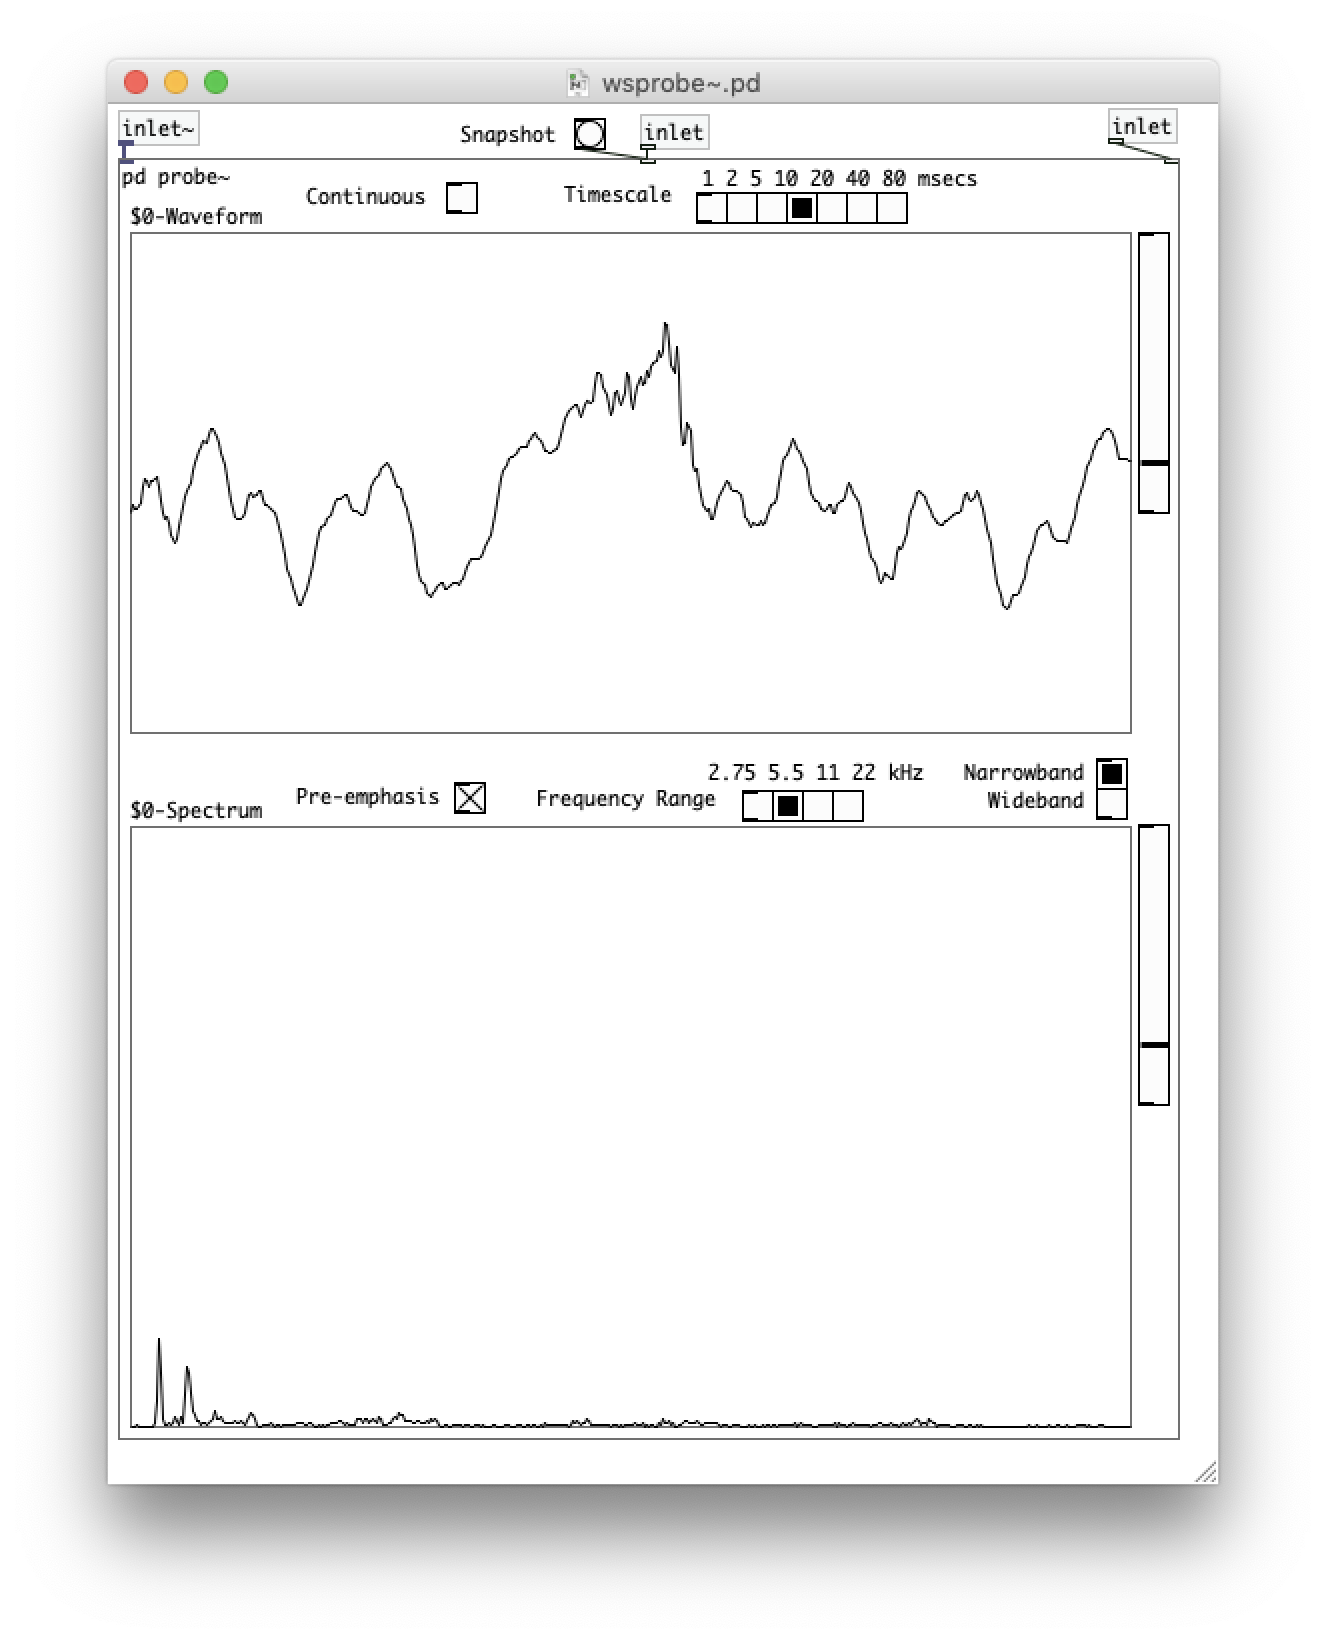
\includegraphics[width=0.6\textwidth]{q1-voiced.png}}
\end{figure}
\end{mdframed}
\vspace*{\baselineskip}

{\color{red}{\bfseries QUESTION \myq\  \emph{(worth up to 5 marks)}}\\Which sounds are most affected when the low-pass cut-off frequency is set to around 500 Hz - vowels or consonants - and why?}
\\
\begin{mdframed}
Consonants are most affected. This is because vowels are voiced which have lower frequencies (250Hz to 1000Hz). Consonants on the other hand have higher frequencies (1500Hz to 6000Hz). The low-pass filter allows through lower frequencies (vowels) while severely damping higher frequencies (consonants). However, you could still hear dampened consonants as the filter doesn't entirely cut-off the frequencies but rather heavily dampen them at a rate of 6dB per octave.
\end{mdframed}
\vspace*{\baselineskip}

{\color{red}{\bfseries QUESTION \myq\ \emph{(worth up to 5 marks)}}\\How is it that the speech is still quite intelligible when the high-pass cut-off frequency is set to 10 kHz?}
\\
\begin{mdframed}
The higher the cut-off frequency, the more aggressive the dampening of the lower frequencies which results in a quieter less-noisy speech signal. A high-pass filter is mainly used for noise cancellation. It's given a roll-off frequency (Also known as the cut-off frequency). PD implements a one-pole high-pass filter with a roll-off rate of 6dB per octave. 
\end{mdframed}
\vspace*{\baselineskip}

{\color{red}{\bfseries QUESTION \myq\ \emph{(worth up to 5 marks)}}\\COM3502-4502-6502: The \texttt{[GraphicEqualiser$\sim$]} object uses an FFT internally; what does FFT stand for and what does an FFT do?\\COM4502-6502 ONLY: What is a DFT and how is it different from an FFT?}
\\
\begin{mdframed}
FFT stands for Fast Fourier Transform. It separates a complex sound signal into it's individual sinusoidal components each with their own amplitude and phase. FFT is an efficient variant of DFT (Discrete Fourier Transform) where it's complexity is $nLogn$ instead of $n^2$.
\end{mdframed}
\vspace*{\baselineskip}

{\color{red}{\bfseries QUESTION \myq\ \emph{(worth up to 10 marks)}}\\With \texttt{speed = 50} and \texttt{depth = 0.5}, what are the minimum and maximum amplitudes of your LFO output, and how do they vary with changes in these two settings?  Also, please provide two screenshots: (a) your \texttt{[LFO$\sim$-help]} object and (b) the internal structure of your \texttt{[LFO$\sim$]} object.}
\\
\begin{mdframed}
The minimum amplitude is -0.5m and the maximum is 0.5m. Varying the speed changes the frequency proportionality. Varying the depth changes the amplitude proportionality. 

\begin{figure}[H]
  \begin{center}
    \frame{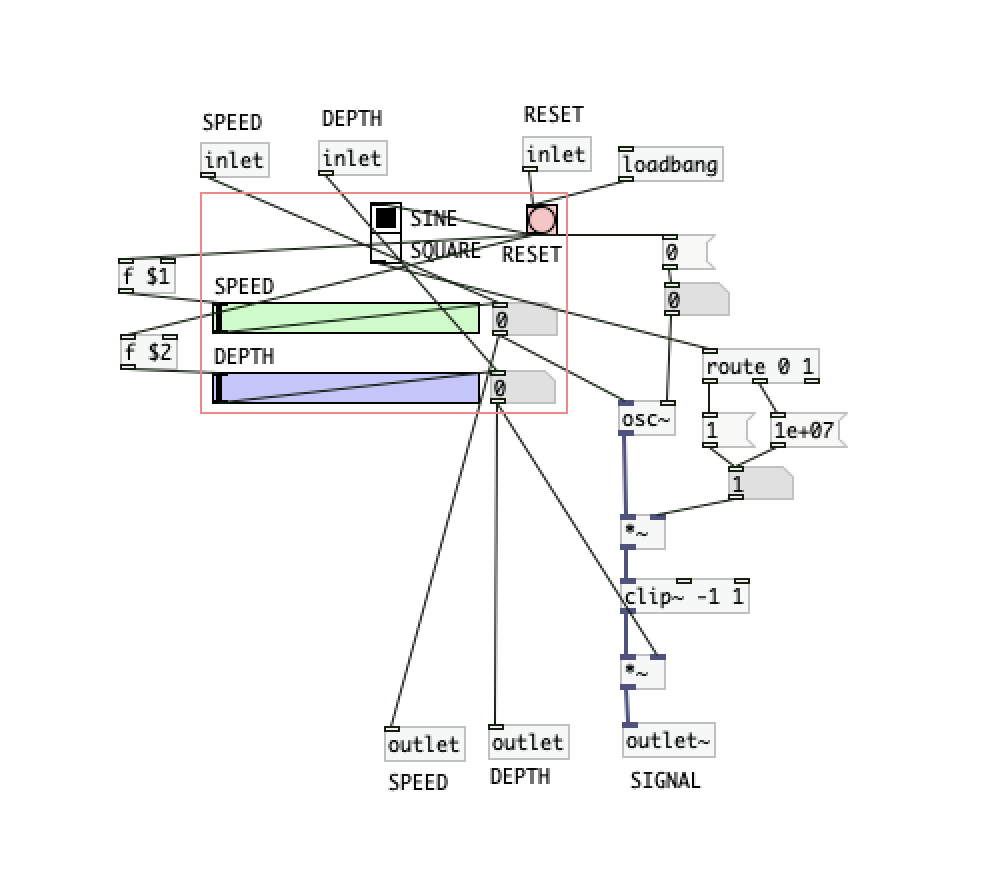
\includegraphics[width=0.6\textwidth]{LFO.png}}
  \end{center} 
\end{figure}
\begin{figure}[H]
  \begin{center}
    \frame{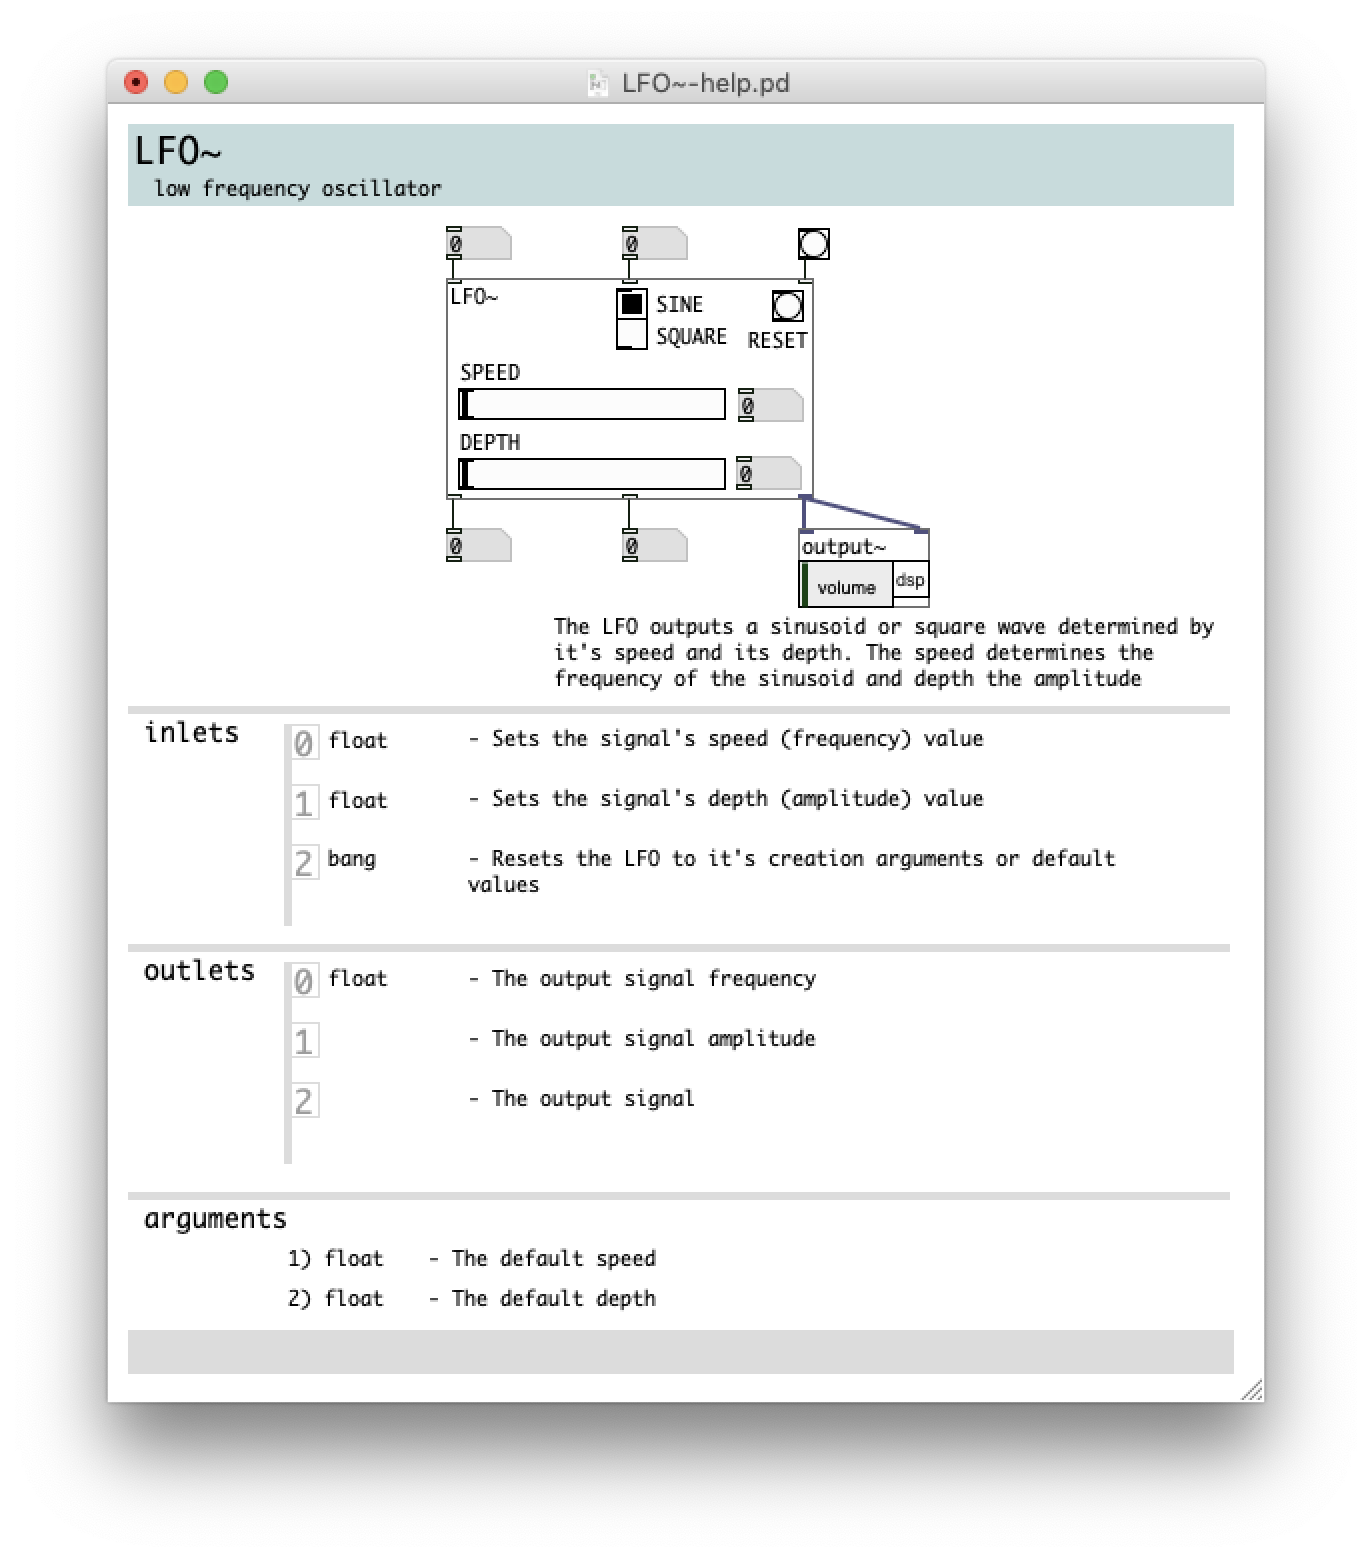
\includegraphics[width=0.6\textwidth]{LFOHelp.png}}
  \end{center}
\end{figure}
\end{mdframed}
\vspace*{\baselineskip}

{\color{red}{\bfseries QUESTION \myq\ \emph{(worth up to 5 marks)}}\\In your own words\footnote{I.e.\ do not plagiarise from Wikipedia.}, why is this effect known as `ring modulation'?}
\\
\begin{mdframed}
Ring modulation is a form of amplitude modulation within the audible range of frequencies. The effect is known as "Ring modulation" due to the 'ring' of diodes in the center of the circuit used to create this effect. The effect multiplies the two signals together which produces a signal equivalent to the sums and differences of the frequencies in both signals.
\end{mdframed}
\vspace*{\baselineskip}

{\color{red}{\bfseries QUESTION \myq\ \emph{(worth up to 5 marks)}}\\Why is SSB commonly used in long-distance radio voice communications?}
\\
\begin{mdframed}
Amplitude modulation on a signal results in two sidebands. One of them is higher in frequency while the other is lower in frequency. To create a SSB, one of these two sidebands (most commonly the one lower in frequency which is known as the lower sideband) along with the carrier wave are removed. This results in an improved and more efficient signal in regards to power and spectrum which is ideal for long-distance radio voice communications.\end{mdframed}
\vspace*{\baselineskip}

{\color{red}{\bfseries QUESTION \myq\ (\emph{worth up to 5 marks)}}\\COM3502-4502-6502: Why can the voice be shifted up in frequency much further than it can be shifted down in frequency before it becomes severely distorted?  \emph{Hint: look at \texttt{[wsprobe$\sim$]}.}\\COM4502-6502 ONLY: Your frequency shifter changes all the frequencies present in an input signal. How might it be possible to change the pitch of a voice \emph{without} altering the formant frequencies?}
\\
\begin{mdframed}
The voice can be shifted up higher because the human voice ranges within lower frequencies. The human voice ranges between 85Hz to 255Hz. Shifting down the signal quickly results in an output that is outside of the human range of hearing (20Hz to 20,000Hz) whereas shifting up results in a signal that is still within the human range of hearing for much more frequencies. 
\end{mdframed}
\vspace*{\baselineskip}

{\color{red}{\bfseries QUESTION \myq\ \emph{(worth up to 5 marks)}}\\In a practical system, why is it important to keep the feedback gain less than 1?}
\\
\begin{mdframed}
Feedback being applied is known as "Positive feedback". Such feedback results in an overall increased signal in terms of magnitude. On increasing the gain above 1, exponential growth occurs, parameters reach extreme magnitudes causes chaotic extreme behaviour. \texttt{[wsprobe$\sim$]} has shown that the harmonics have increased significantly while the waveform has shown a massive increase in frequency and amplitude. This is why positive feedback tends to cause system instability.
\end{mdframed}
\vspace*{\baselineskip}

{\color{red}{\bfseries QUESTION \myq\ \emph{(worth up to 50 marks\footnote{25 for functionality, 15 for design/layout, 5 for \texttt{Pd} features, 5 for innovations})}}\\Please provide a short\footnote{no more than 200 words} description of the operation of your \texttt{[VoiceChanger]} application, together with a screenshot of your final GUI.}
\\
\begin{mdframed}
The \texttt{[VoiceChanger]} output is controlled by the 'MASTER VOLUME' dial. Adjusting this dial will increase and decrease the volume accordingly. Similarly, each filter and effect is controlled by their own dial. This controls the mix between the signal before the effect and after the effect. Effects are relevantly categorized and they're all connected together allowing custom combinations when used in conjunction with the effect dials. To demonstrate different settings, a number of presets have been supplied.
\begin{itemize}
	\item Inputs
		\begin{enumerate}
			\item Live signal (Caution: Use Headphones)
			\item File input
		\end{enumerate}
	\item Output:
		\begin{enumerate}
			\item Processed signal
		\end{enumerate}
	\item Filters:
		\begin{enumerate}
			\item Low-pass
			\item High-pass
			\item Band-pass
		\end{enumerate}
	\item Effects:
		\begin{enumerate}
			\item Frequency Shifter
			\item Vibrato
			\item Tremolo
			\item Ring Modulation
			\item Delay
			\item Reverberation
			\item Flanger
		\end{enumerate}
	\item Presets:
		\begin{enumerate}
			\item C3P0 
			\item Dalek
			\item Robot
			\item Phasing (Comb filtering)
			\item Reverberant room
			\item Echo
			\item Underwater
			\item Gollum
		\end{enumerate}
\end{itemize}
\begin{figure}[H]
  \begin{center}
    \frame{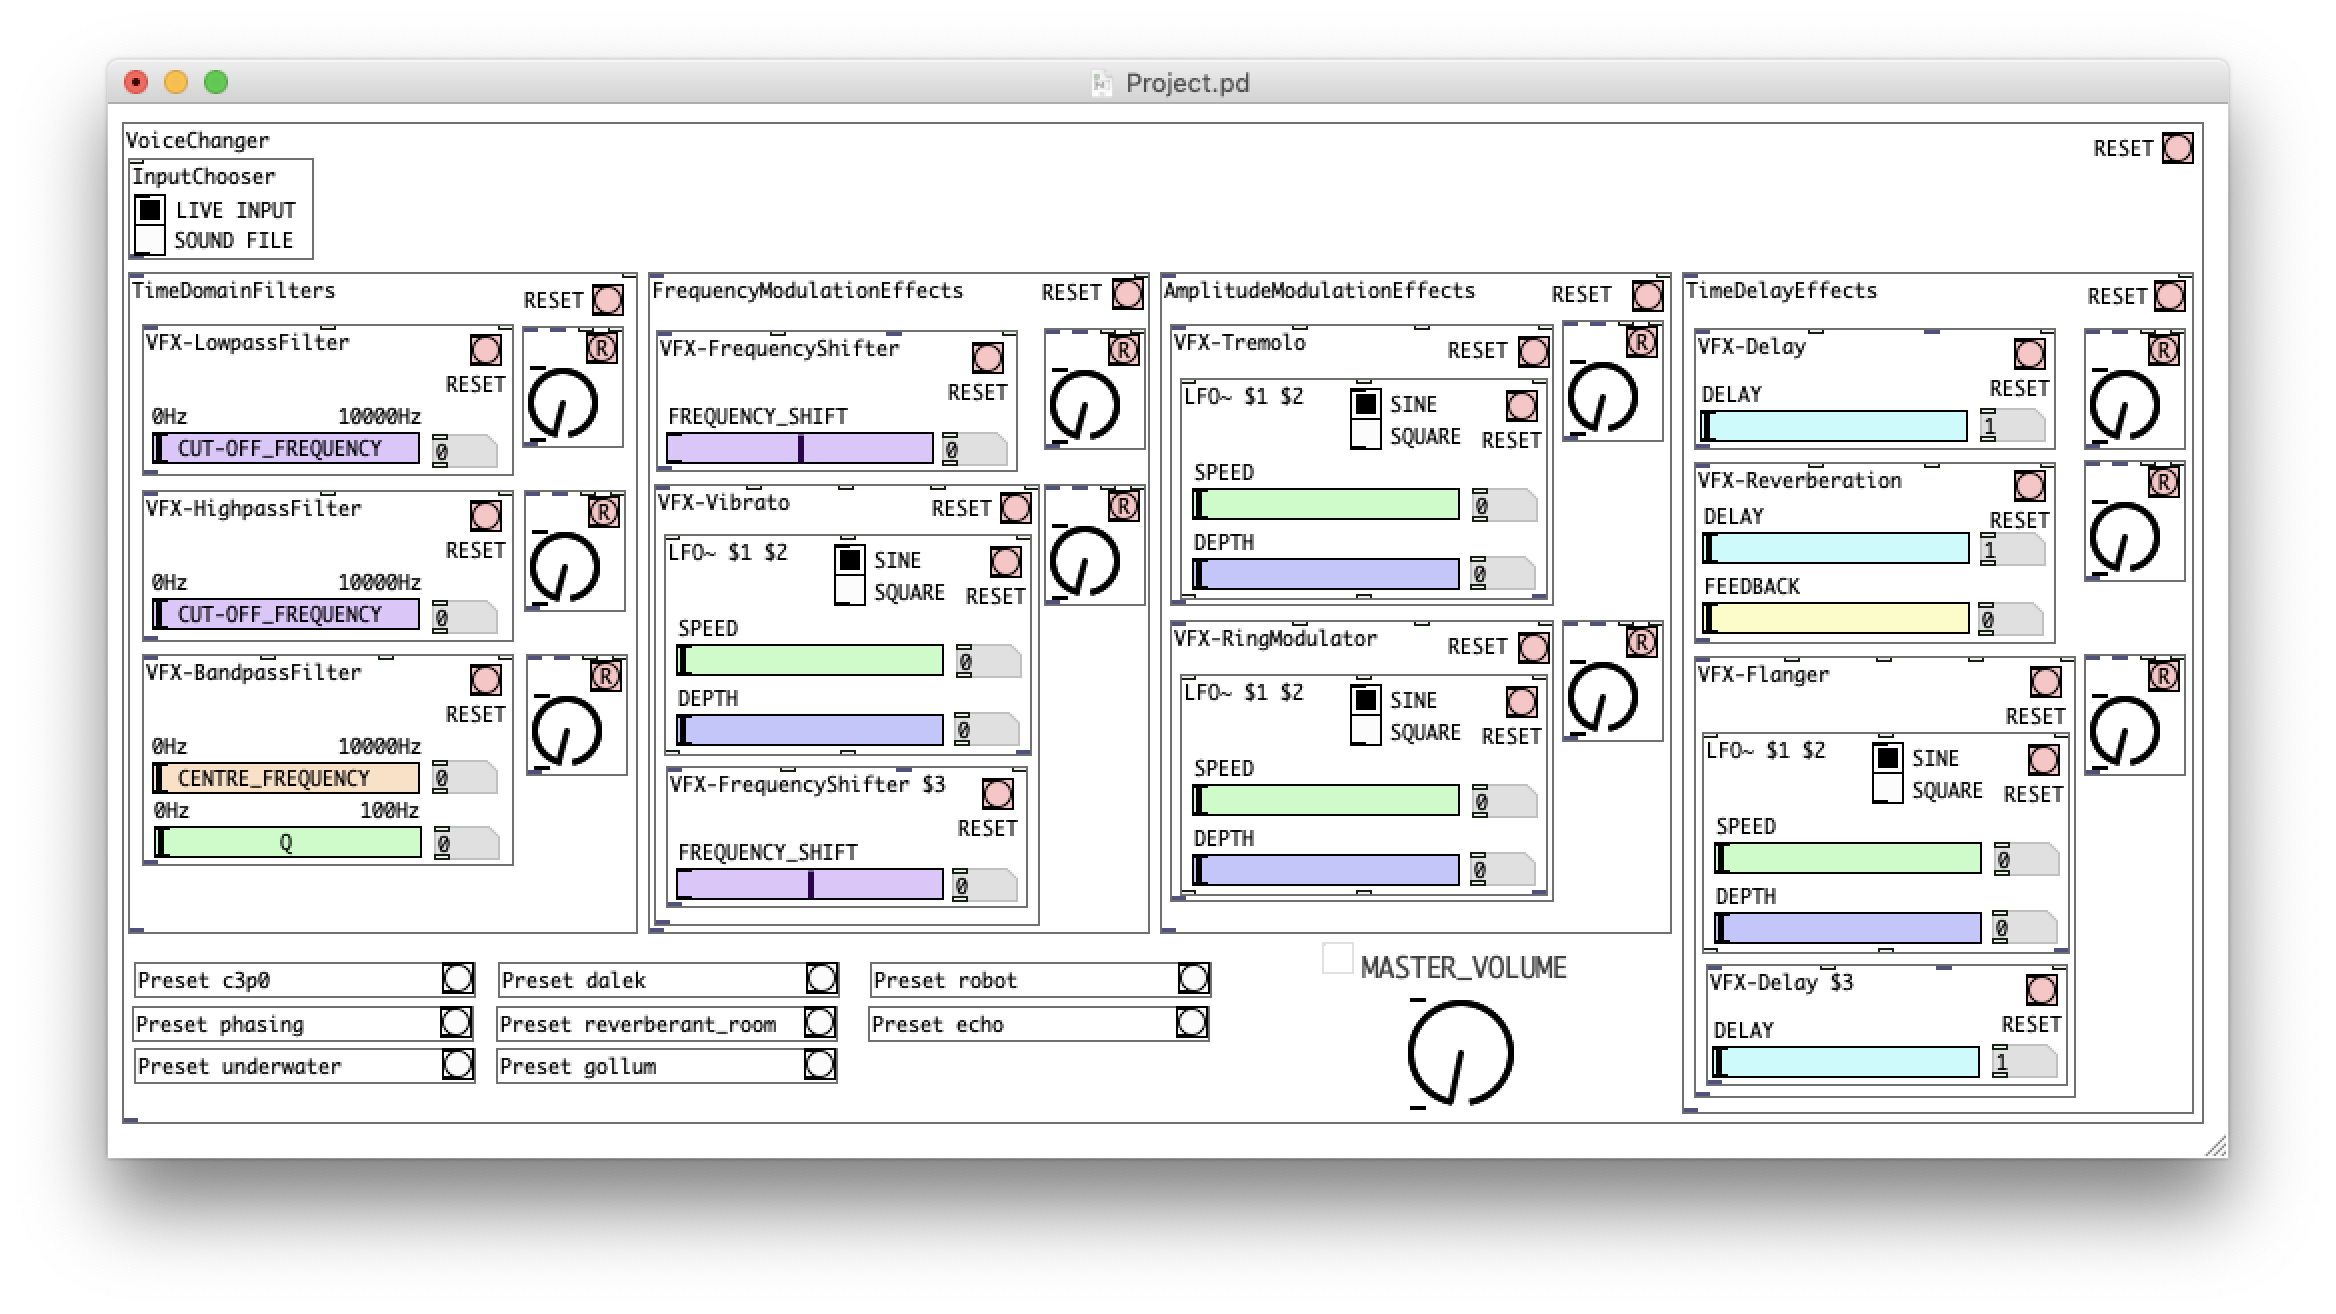
\includegraphics[width=1\textwidth]{VoiceChanger.png}}
  \end{center}
\end{figure}
\end{mdframed}
\vspace*{\baselineskip}

\end{document}